\documentclass[sigconf]{acmart}

\usepackage{pgfplots}
\usepackage{placeins}  % Required for \FloatBarrier
\pgfplotsset{compat=1.17}

%%
%% \BibTeX command to typeset BibTeX logo in the docs
\AtBeginDocument{%
  \providecommand\BibTeX{{%
    \normalfont B\kern-0.5em{\scshape i\kern-0.25em b}\kern-0.8em\TeX}}}

%% Rights management information.  This information is sent to you
%% when you complete the rights form.  These commands have SAMPLE
%% values in them; it is your responsibility as an author to replace
%% the commands and values with those provided to you when you
%% complete the rights form.
\setcopyright{acmcopyright}
\copyrightyear{2023}
\acmYear{2023}
\acmDOI{XXXXXXX.XXXXXXX}

%% These commands are for a PROCEEDINGS abstract or paper.
\acmConference[Conference acronym 'XX]{Make sure to enter the correct
  conference title from your rights confirmation emai}{June 03--05,
  2018}{Woodstock, NY}
\acmPrice{15.00}
\acmISBN{978-1-4503-XXXX-X/18/06}


%%
%% Submission ID.
%% Use this when submitting an article to a sponsored event. You'll
%% receive a unique submission ID from the organizers
%% of the event, and this ID should be used as the parameter to this command.
%%\acmSubmissionID{123-A56-BU3}

%%
%% For managing citations, it is recommended to use bibliography
%% files in BibTeX format.
%%
%% You can then either use BibTeX with the ACM-Reference-Format style,
%% or BibLaTeX with the acmnumeric or acmauthoryear sytles, that include
%% support for advanced citation of software artefact from the
%% biblatex-software package, also separately available on CTAN.
%%
%% Look at the sample-*-biblatex.tex files for templates showcasing
%% the biblatex styles.
%%

%%
%% The majority of ACM publications use numbered citations and
%% references.  The command \citestyle{authoryear} switches to the
%% "author year" style.
%%
%% If you are preparing content for an event
%% sponsored by ACM SIGGRAPH, you must use the "author year" style of
%% citations and references.
%% Uncommenting
%% the next command will enable that style.
%%\citestyle{acmauthoryear}

%%
%% end of the preamble, start of the body of the document source.
\begin{document}

%%
%% The "title" command has an optional parameter,
%% allowing the author to define a "short title" to be used in page headers.
\title{Dependability Analysis - Apache commons-imaging library}

%%
%% The "author" command and its associated commands are used to define
%% the authors and their affiliations.
%% Of note is the shared affiliation of the first two authors, and the
%% "authornote" and "authornotemark" commands
%% used to denote shared contribution to the research.
\author{Julian Alexis Orcinoli}
\authornote{All authors contributed equally to this research.}
\affiliation{%
  \institution{Università degli Studi di Salerno}
  \city{Fisciano}
  \state{Salerno}
  \country{Italy}
  \postcode{84084}
}
\email{j.orcinoli@studenti.unisa.it}

\author{Santiago Morales Henao}
\authornote{All authors contributed equally to this research.}
\affiliation{%
  \institution{Università degli Studi di Salerno}
  \city{Fisciano}
  \state{Salerno}
  \country{Italy}
  \postcode{84084}
}
\email{s.moraleshenao@studenti.unisa.it}

\author{Franco Nicolás Merenda}
\authornote{All authors contributed equally to this research.}
\affiliation{%
  \institution{Università degli Studi di Salerno}
  \city{Fisciano}
  \state{Salerno}
  \country{Italy}
  \postcode{84084}
}
\email{f.merenda2@studenti.unisa.it}


%%
%% By default, the full list of authors will be used in the page
%% headers. Often, this list is too long, and will overlap
%% other information printed in the page headers. This command allows
%% the author to define a more concise list
%% of authors' names for this purpose.
\renewcommand{\shortauthors}{Julian A. Orcinoli, Merenda F. Nicolas, and Santiago M. Henao}

%%
%% The abstract is a short summary of the work to be presented in the
%% article.
\begin{abstract}
  This paper presents a comprehensive analysis of software dependability in the context of the Apache Commons Imaging project, a vital component of the Apache Commons IO ecosystem. The study employs a multifaceted approach, leveraging software analytics, testing tools, and vulnerability assessment techniques to evaluate and enhance the dependability and code quality of the project.

  The analysis begins with an exploration of SonarCloud, delving into the identification and resolution of bugs. Subsequently, various software testing tools, including JaCoCo, CodeCov, PiTest, and EvoSuite, are employed to assess code coverage, mutation testing, and automated test case generation. The study extends to vulnerability checking using OWASP Dependability Checker and FindSecBugs.
  
  Results showcase improvements in code quality, increased code coverage, and the identification and remediation of software vulnerabilities. The paper contributes valuable insights into the efficacy of diverse tools and methodologies in ensuring software dependability. Through this investigation, we aim to provide a nuanced understanding of the strengths and limitations of each approach, offering guidance for future endeavors in the pursuit of reliable and robust software systems.
\end{abstract}

%%
%% The code below is generated by the tool at http://dl.acm.org/ccs.cfm.
%% Please copy and paste the code instead of the example below.
%%
\begin{CCSXML}
<ccs2012>
   <concept>
       <concept_id>10011007.10011074.10011099.10011102.10011103</concept_id>
       <concept_desc>Software and its engineering~Software testing and debugging</concept_desc>
       <concept_significance>500</concept_significance>
    </concept>
    <concept>
       <concept_id>10011007.10011006.10011073</concept_id>
       <concept_desc>Software and its engineering~Software maintenance tools</concept_desc>
       <concept_significance>500</concept_significance>
   </concept>
   <concept>
       <concept_id>10011007.10011074.10011134.10003559</concept_id>
       <concept_desc>Software and its engineering~Open source model</concept_desc>
       <concept_significance>300</concept_significance>
   </concept>

 </ccs2012>
\end{CCSXML}

\ccsdesc[500]{Software and its engineering~Software testing and debugging}
\ccsdesc[500]{Software and its engineering~Software maintenance tools}
\ccsdesc[300]{Software and its engineering~Open source model}


%%
%% Keywords. The author(s) should pick words that accurately describe
%% the work being presented. Separate the keywords with commas.
\keywords{Software Dependability, Apache Commons Imaging, Software Analytics, SonarCloud, Software Testing Tools, Code Coverage, JaCoCo, CodeCov, Mutation Testing, PiTest, Java Microbenchmark Harness, JMH,  Automated Test Case Generation, EvoSuite, Software Vulnerabilities, OWASP Dependability Checker, FindSecBugs, Bug Fixing, Code Quality, Software Engineering}

%% \received{20 February 2007}
%% \received[revised]{12 March 2009}
%% \received[accepted]{5 June 2009}

%%
%% This command processes the author and affiliation and title
%% information and builds the first part of the formatted document.
\maketitle

\section{Introduction}
The evolution of software dependability, intrinsic to modern computing, spans from mainframes to interconnected networks, broadening its focus on reliability, fault tolerance, security, and safety. Pioneering works in the 1980s emphasized redundancy techniques like Triple-Modular Redundancy. Shifting to the 1990s, the spotlight turned to security and safety, addressing cyber threats in banking and hazards prevention in healthcare software. Software dependability encompasses reliability, availability, safety, security, maintainability, and fault tolerance. Recent years witnessed increased complexity in cloud computing and IoT, necessitating innovative approaches. Avizienis, Laprie, Randell, and Landwehr emphasized the role of fault tolerance. Ongoing contributions underscore the evolution of these principles. As technology advances, software dependability will continue to evolve, balancing functionality, performance, and societal impact in interconnected systems.

In the contemporary technological landscape, software systems play a pivotal role across diverse domains, shaping both personal and societal interactions. The escalating reliance on software underscores the critical need for dependability in these systems. This paper embarks on a comprehensive exploration of software dependability, covering diverse aspects such as project analysis, testing tools, and vulnerability checks.

Commencing with an overview of Apache Commons Imaging \cite{apache-commons-imaging}, a project within the Apache Commons IO ecosystem, this paper sets the foundation for subsequent analyses. Insights into the project's structure are provided, offering context to the broader discussions on software dependability.

Moving forward, Software Analytics takes center stage, delving into bug identification and fixes. This meticulous analysis provides a nuanced understanding of software quality and dependability through advanced analytical tools.

The exploration of Software Testing Tools follows, encompassing crucial tools like JaCoCo and CodeCov. The analysis spans code coverage evaluations before and after bug fixes, augmented by insights from Mutation Testing and Java Microbenchmark Harness.

The next section focuses on the Automated Generation of Test Cases, using a tool named EvoSuite. This section probes the efficacy of these tools in generating meaningful test cases, aligning with the overarching theme of software dependability.

The critical dimension of Software Vulnerabilities is dissected, providing a brief overview of tools like OWASP Dependability Checker and FindSecBugs. Practical insights into running these tools, fixing identified bugs, and engaging in insightful discussions enrich this section.

The ensuing discussion section serves as a platform to scrutinize findings, highlight encountered challenges, and address pivotal issues in the realm of software dependability.

In conclusion, this paper synthesizes a multifaceted exploration of software dependability, transcending traditional boundaries. Covering project analysis, analytics, testing tools, and vulnerability checks, it encapsulates the essence of reliability, security, and robustness in software systems.

\subsection{Apache Commons Imaging}
Apache Commons Imaging is a powerful open-source Java library that resides within the Apache Commons project. This library focuses on simplifying the complexities of image processing for Java developers. Boasting support for a diverse range of image formats, including popular ones such as JPEG, PNG, GIF, BMP, and TIFF, provides a versatile toolkit for developers working with images.

One notable aspect of Apache Commons Imaging is its commitment to cross-platform compatibility, ensuring that developers can seamlessly integrate the library into various operating systems and environments. The project maintains an active and collaborative community, welcoming contributions and fostering an environment conducive to continual improvement.

In conclusion, Apache Commons Imaging stands out as an essential tool for Java developers engaged in image-related tasks. Its extensive format support, versatile manipulation capabilities, and commitment to collaboration make it a reliable choice for projects requiring robust image processing functionality.

\section{SonarCloud}

\begin{figure}[h!]
    \centering
    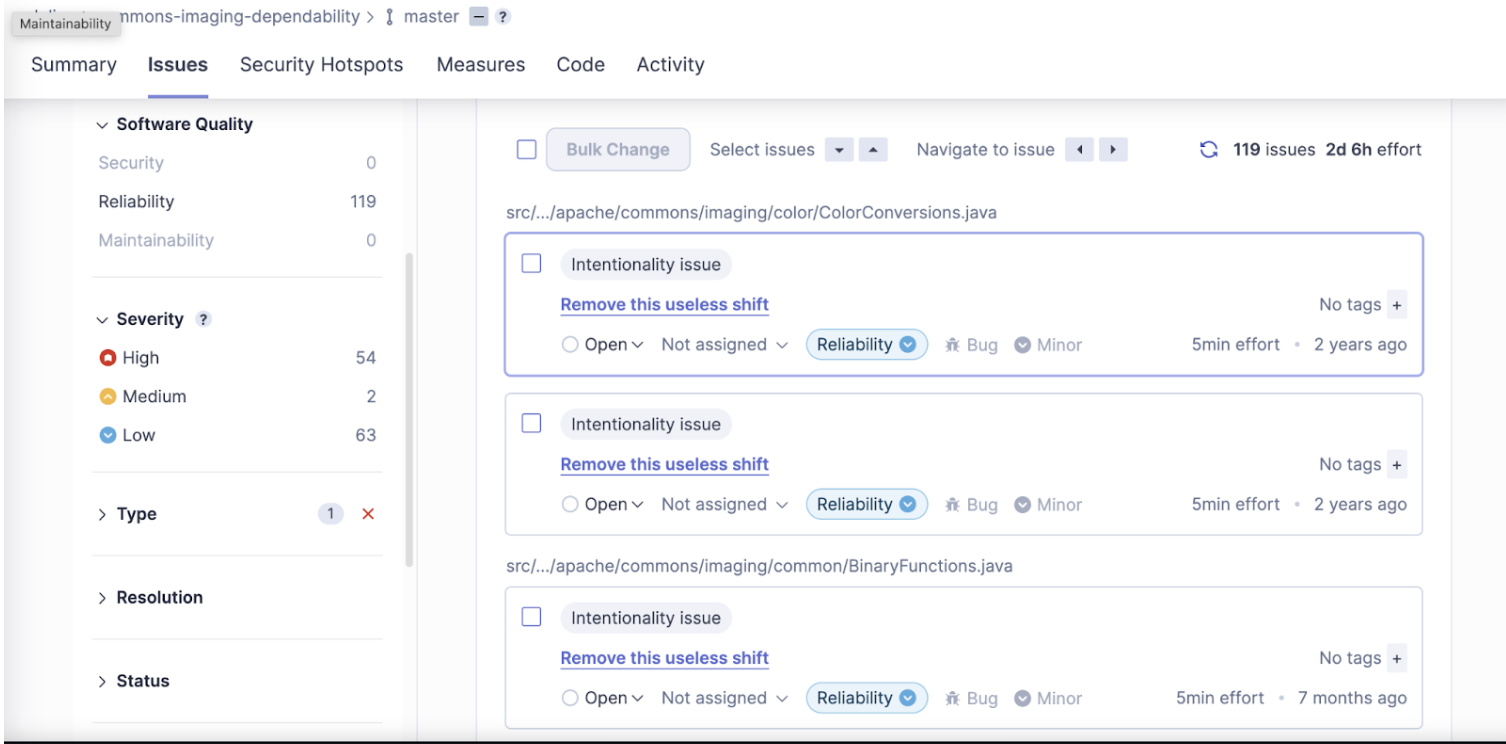
\includegraphics[width=1\linewidth]{reportSonarCloud.png}
    \caption{Report before fix}
    \label{fig:enter-label}
\end{figure}


\subsection{Analyzing SonarCloud}

After analyzing the commons-imaging-dependability project on SonarCloud, we found the following issues in the code:

\textbf{High → 54}

In the high category, several errors are related to divisions where the divisor is not checked for the possibility of being 0. Therefore, if the divisor is 0, the code would throw an exception. There are also errors of the type where referencing a static member of a subclass from its parent during class initialization makes the code more fragile and prone to future errors. The program's execution will largely depend on the order of class and static member initialization.

\textbf{Medium → 2}

In the medium category, there are only 2 errors where an attempt is made to get the length of a palette that could be null.

\textbf{Low → 63}

Out of these 63 errors, most are related to the suggestion to remove a left shift, explaining that an int is a 32-bit variable and specifying that shifting an int by 32 is the same as shifting by 0, and shifting by 33 is the same as shifting by 1. Additionally, there are some errors related to number casting.

\subsection{Bugs Fixed}

To organize our tasks based on the errors found in \textbf{SonarCloud}, we created tasks in \textbf{JIRA}, and each of them was assigned to the three members of the group. We attempted to address the majority of the 119 issues related to reliability, of which we were able to fix XX.

\begin{figure}[h!]
    \centering
    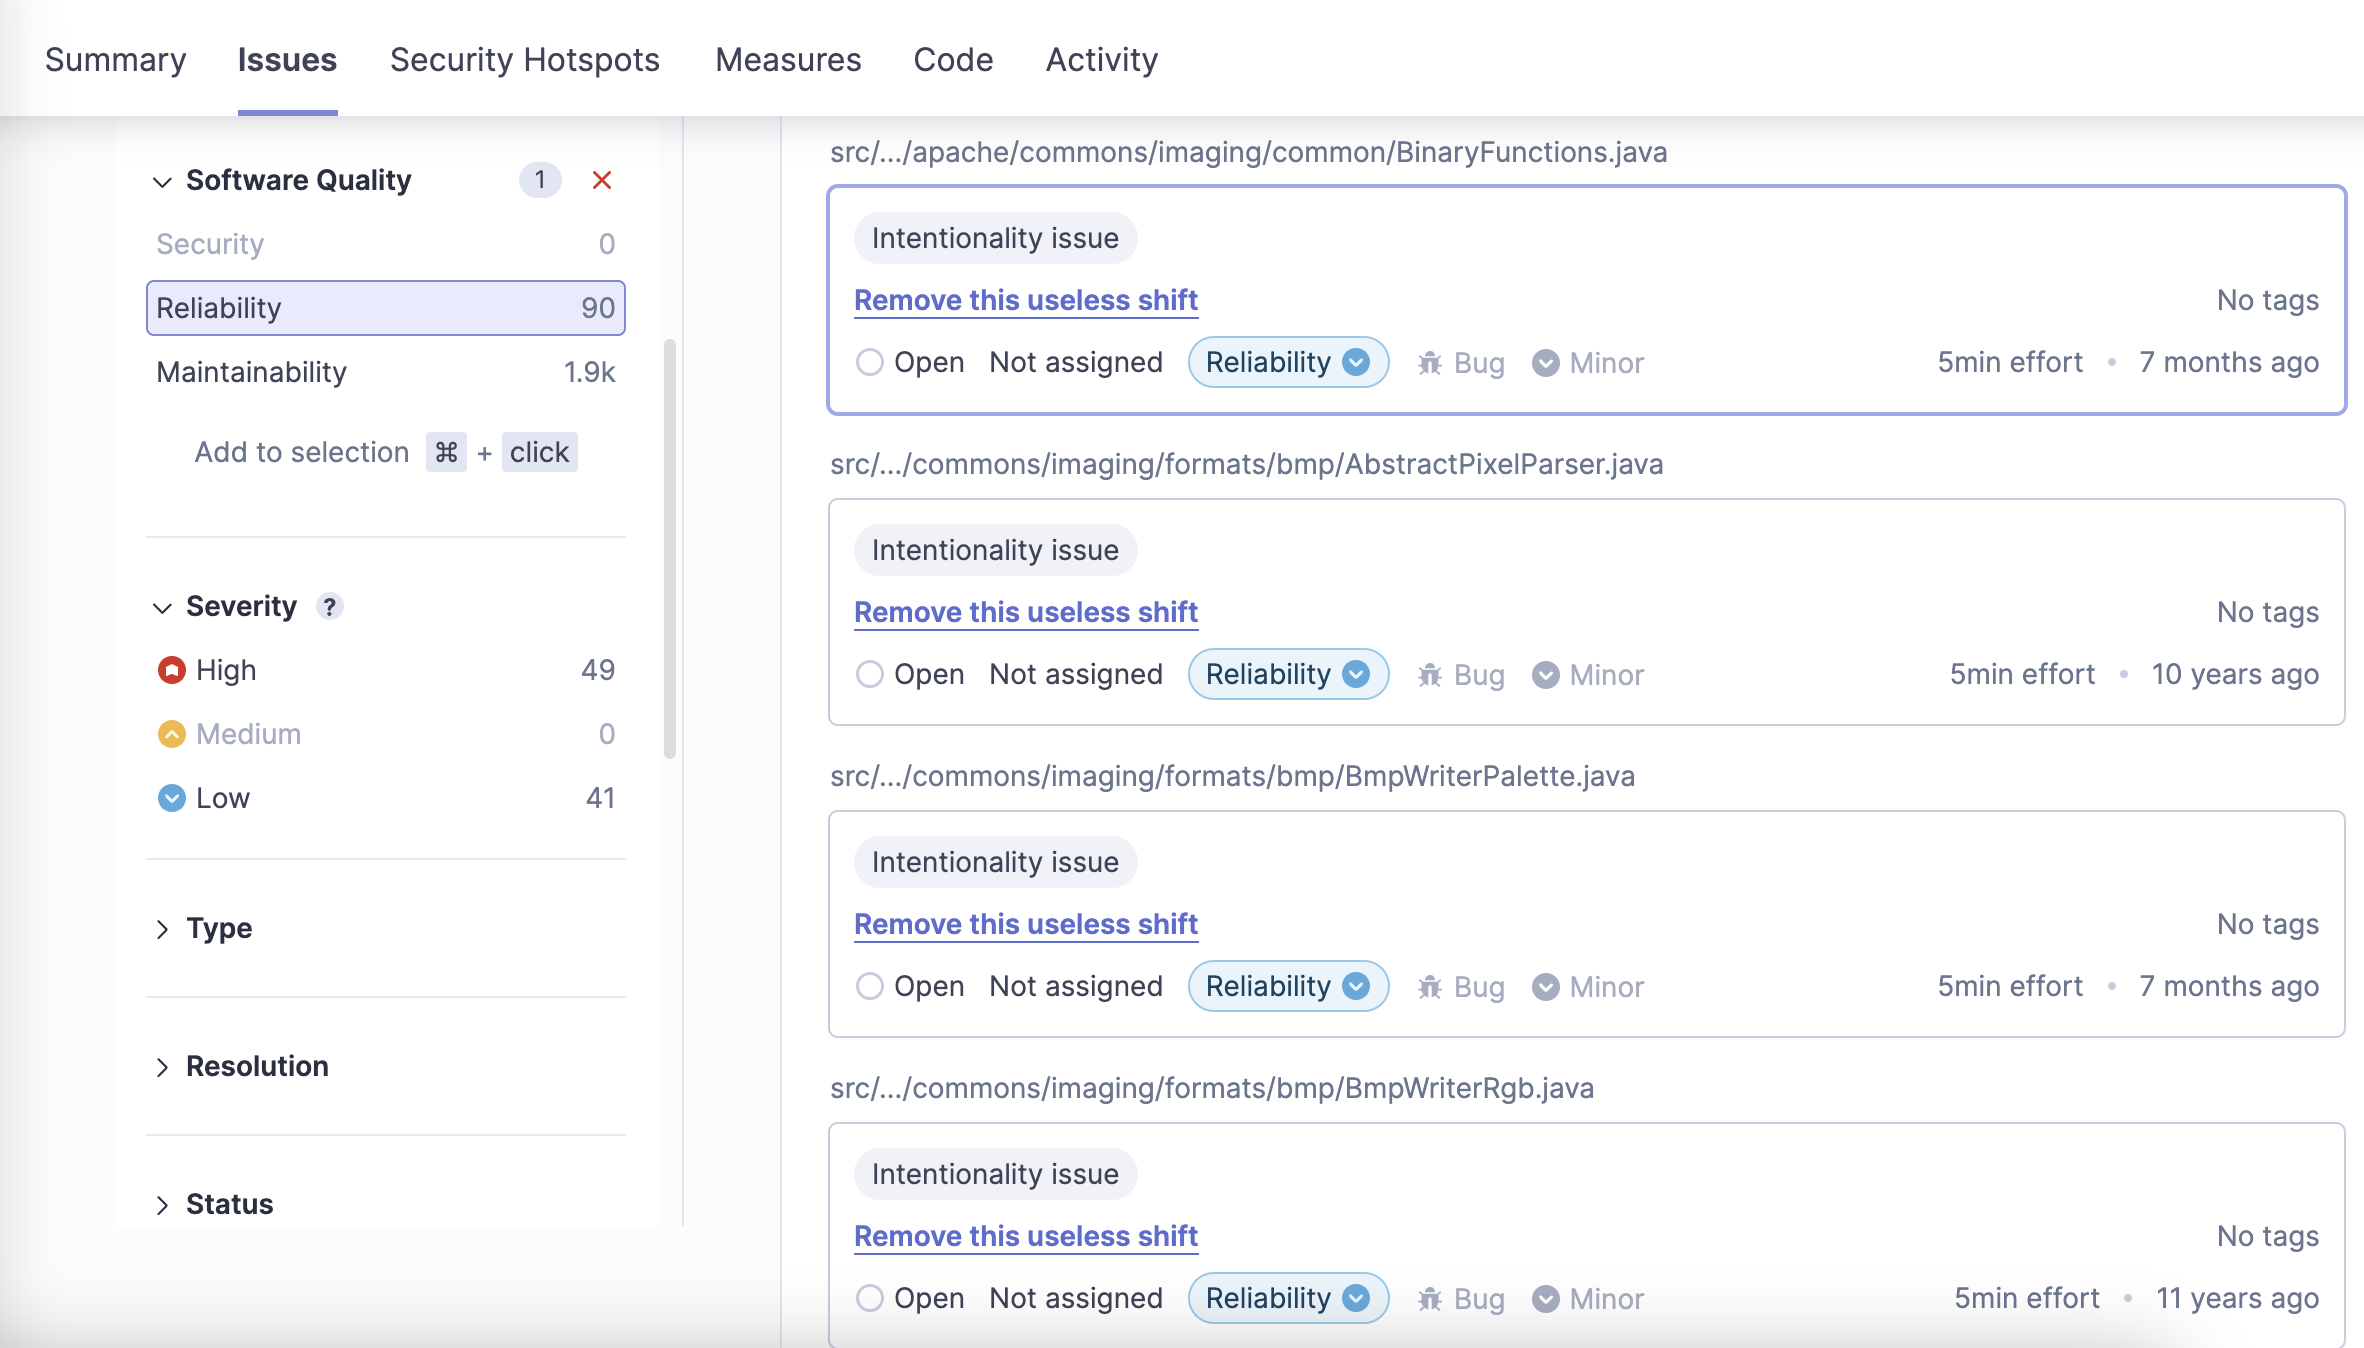
\includegraphics[width=1\linewidth]{reportSonarCloudFixed.png}
    \caption{Bugs Fixed}
    \label{fig:enter-label}
\end{figure}


\section{Software Testing Tools}

To measure and improve the robustness of the Apache Commons Imaging project's dependability, this section focuses on three key testing tools. First, we delve into the realm of code coverage using JaCoCo and CodeCov, unraveling their importance and impact. Following that, we explore mutation testing with PiTest, evaluating the resilience of test cases. The journey concludes with Java Microbenchmark Harness, providing insights into performance characteristics. Together, these tools form a robust arsenal to fortify and enhance the project's reliability.

\subsection{Code Coverage - JaCoCo}
JaCoCo \cite{jacoco} (Java Code Coverage) serves as a vital tool in assessing code coverage for Java applications, offering valuable insights into the extent of code execution during testing. It generates comprehensive reports that pinpoint the specific portions of the code exercised by tests.

Our investigation utilizing JaCoCo revealed a baseline of 77\% Instructions Coverage and 63\% Branches Coverage. This includes specific metrics such as 2448/6213 missed cyclomatic complexities, 3931/17299 missed lines, 511/2539 missed methods, and 16/431 missed classes.

A notable feature of JaCoCo lies in its ability to set a minimum expected coverage. This proactive measure ensures that code changes maintain a predefined level of coverage \cite{jacoco-check-mojo}, contributing significantly to the overall robustness of the project.

\subsection{Code Coverage - CodeCov}
CodeCov \cite{codecov} emerges as an instrumental tool, orchestrating a meticulous examination of code coverage within the Apache Commons Imaging project. This sophisticated platform specializes in unraveling the intricacies of test suite effectiveness.

\textbf{Key Metrics:}
\begin{enumerate}
    \item \textbf{Overall Code Coverage:} Our CodeCov analysis reveals a comprehensive code coverage of 71.17\% across the entirety of the project. This quantitative metric serves as a substantive indicator of the extent to which our test suites engage with the codebase.
    
    \item \textbf{Files with Lower Coverage Rates (In use with Below 0\%):}
    \begin{itemize}
        \item \texttt ColorTools.java
        \item \texttt PixelDensity.java
        \item \texttt DataParserBitmap.java
        \item \texttt TagInfoSLongs.java
        \item \texttt ColorTools.java
        \item \texttt PbmWriter.java
        \item \texttt PgmWriter.java
        \item \texttt UncompressedDataReader.java
        \item \texttt ScanExpediterInterlaced.java
        \item \texttt PhotometricInterpreterCieLab.java
        \item \texttt PhotometricInterpreterYCbCr.java
        \item \texttt FieldTypeFloat.java
    \end{itemize}
    
    \item \textbf{Line Coverage:} A granular examination exposes that among the 17,299 lines constituting the project, the project covers 12,311 lines.
\end{enumerate}

Following the addition of targeted tests aimed at addressing files with 0\% coverage, the overall code coverage has substantially increased to 71.82\%. Out of a total of 17,303 lines, 12,427 are now covered. Notably, certain sections of the code remain only partially covered, emphasizing the ongoing commitment to fortify the software's robustness and reliability.


\subsection{Mutation Testing - PiTest}
TODO

\subsection{Java Microbenchmark Harness}
JMH\cite{jmh} is a powerful tool specifically designed for benchmarking Java code, allowing us to meticulously analyze the performance of our compression algorithms.

In the context of our image management project, an in-depth analysis of CPU-intensive image formats has revealed TIFF and WebP as the most demanding formats in terms of system resources. Following this, a detailed examination of test durations highlighted a specific, time-consuming scenario (\texttt{org.apache.commons.\\imaging.formats.tiff.TiffRoundtripTest.test}): the compression of TIFF images utilizing various algorithms (\texttt{TIFF\_COMPRESSION\_\\LZW}, \texttt{TIFF\_COMPRESSION\_PACKBITS}, \texttt{TIFF\_COMPRESSION\_DEFLATE\_\\ADOBE}, and \texttt{Uncompressed}).

\subsubsection{Environment and Program Execution Specifications}

\textbf{Hardware Specifications:}
\begin{itemize}
  \item CPU: Apple M1 Pro (2021)
  \item OS: MacOS Sonoma 14.2.1
  \item RAM: 16GB unified memory
\end{itemize}

\textbf{Program Execution Specifications (for report):}
\begin{itemize}
  \item \texttt{OpenJDK version "1.8.0\_392"}
  \item \texttt{OpenJDK Runtime Environment Corretto-8.392.08.1 (build 1.8.0\_392-b08)}
  \item \texttt{OpenJDK 64-Bit Server VM Corretto-8.392.08.1 (build 25.392-b08, mixed mode)}
\end{itemize}

\subsubsection{Results}
To further explore the performance of each compression algorithm, each algorithm was applied separately to the same set of images, conducting a benchmark, that yielded the following results: \vspace{12pt}

\textbf{Before Using Concurrency:}
\begin{itemize}
    \item \texttt{TIFF\_COMPRESSION\_DEFLATE\_ADOBE:} Throughput 0.465 $\pm$ 0.006 ops/s
    \item \texttt{TIFF\_COMPRESSION\_LZW:} Throughput 0.216 $\pm$ 0.001 ops/s
    \item \texttt{TIFF\_COMPRESSION\_PACKBITS:} Throughput 1.278 $\pm$ 0.053 ops/s
    \item \texttt{Uncompressed:} Throughput 2.170 $\pm$ 0.019 ops/s
\end{itemize}

Upon thorough review, we identified an opportunity for performance enhancement by introducing parallelism into the compression process. The parallel application of compression algorithms resulted in significant throughput improvements:\vspace{12pt}

\textbf{After Using Concurrency:}
\begin{itemize}
    \item \texttt{TIFF\_COMPRESSION\_DEFLATE\_ADOBE:} Throughput 1.375 $\pm$ 0.012 ops/s (Increase by 196.77\%)
    \item \texttt{TIFF\_COMPRESSION\_LZW:} Throughput 0.774 $\pm$ 0.008 ops/s (Increase by 258.33\%)
    \item \texttt{TIFF\_COMPRESSION\_PACKBITS:} Throughput 2.870 $\pm$ 0.164 ops/s (Increase by 124.61\%)
    \item \texttt{Uncompressed:} Throughput 3.984 $\pm$ 0.066 ops/s (Increase by 83.12\%)
\end{itemize}

\begin{figure}
  \centering
  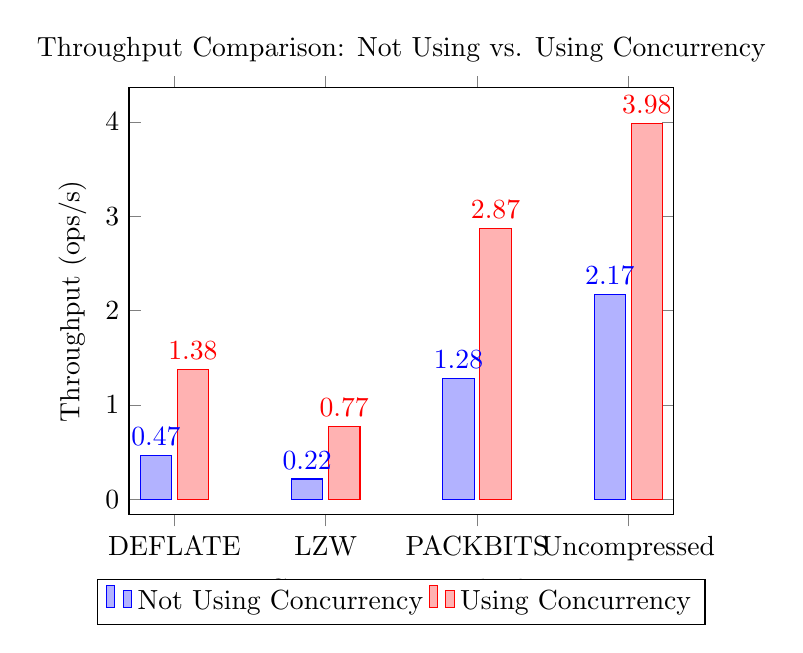
\begin{tikzpicture}
    \begin{axis}[
      ybar,
      bar width=0.4cm,
      width=8.5cm,
      height=7cm,
      xlabel={Compression Methods},
      ylabel={Throughput (ops/s)},
      legend style={at={(0.5,-0.15)}, anchor=north, legend columns=-1},
      symbolic x coords={DEFLATE, LZW, PACKBITS, Uncompressed},
      xtick=data,
      nodes near coords,
      nodes near coords align={vertical},
      title={Throughput Comparison: Not Using vs. Using Concurrency},
    ]
      \addplot coordinates {(DEFLATE, 0.465) (LZW, 0.216) (PACKBITS, 1.278) (Uncompressed, 2.170)};
      \addplot coordinates {(DEFLATE, 1.375) (LZW, 0.774) (PACKBITS, 2.870) (Uncompressed, 3.984)};
      \legend{Not Using Concurrency, Using Concurrency}
    \end{axis}
  \end{tikzpicture}
  \caption{Comparison of Throughput: Not Using vs. Using Concurrency}
  \label{fig:bargraph}
\end{figure}


\FloatBarrier
Beyond benchmark results, we observed a substantial reduction in the tiff test duration, decreasing from 8.4978 $\pm$ 0.0407 seconds ($\pm$0.48\%) to 3.7254 $\pm$ 0.128 seconds ($\pm$3.44\%) by applying compression algorithms to multiple image files in a concurrent way. This notable improvement not only enhances the efficiency of our compression algorithms but also contributes to a more expedited execution of test scenarios.

\subsubsection{Wilcoxon-Mann-Whitney Test and Cliff's Delta}

The Wilcoxon-Mann-Whitney test was performed to compare the two groups: "Not using concurrency" and "Using concurrency."

\begin{itemize}
    \item Test Statistic ($W$): 3
    \item P-value: 0.2
\end{itemize}

\textbf{Decision Rule:} If the p-value is less than or equal to the significance level (\(\alpha\)), typically 0.05, we reject the null hypothesis.

\textbf{Interpretation:} Since the p-value (0.2) is greater than 0.05, there is not enough evidence to reject the null hypothesis. We do not conclude a significant difference between the two groups.


% Cliff's Delta Effect Size
\subsubsection{Cliff's Delta Effect Size}

Cliff's Delta was calculated to assess the effect size between the two groups: "Not using concurrency" and "Using concurrency."

\begin{itemize}
    \item Cliff's Delta: -0.625
\end{itemize}

\textbf{Interpretation:}
\begin{itemize}
    \item A negative value indicates a tendency for lower values in the "Not using concurrency" group compared to the "Using concurrency" group.
    \item The magnitude of -0.625 suggests a moderate-sized effect.
\end{itemize}

\textbf{Conclusion:}
The negative value of Cliff's Delta, with a moderate magnitude, suggests a moderate tendency for lower values in the "Not using concurrency" group compared to the "Using concurrency" group.



\section{Automated Generation of Test Cases}
TODO

\subsection{EvoSuite}
TODO


\section{Software Vulnerabilities}
Software vulnerabilities are weaknesses or flaws in a program that could be exploited by an attacker to compromise the integrity, confidentiality, or availability of the system. These vulnerabilities can exist at various layers of the software, from design errors to implementation flaws. It is crucial to address and fix these vulnerabilities to ensure the security of the software.


Common Types of Vulnerabilities in Apache Commons Imaging:

\begin{itemize}
    \item \textbf{\textit{Data Injection:}} This can occur when external input is not properly filtered or validated, allowing an attacker to inject malicious code.
    
    \item \textbf{\textit{Buffer Overflow:}} This type of vulnerability occurs when the allotted storage capacity for a buffer is exceeded, enabling an attacker to overwrite surrounding memory.
    
    \item \textbf{\textit{Inadequate Validation:}} Lack of input validation can lead to security issues. For example, if a user's authenticity is not verified before executing a critical operation.
    
    \item \textbf{\textit{Authentication and Authorization Issues:}} Failures in authentication or authorization mechanisms may allow unauthorized users to access sensitive resources or functions.
    
    \item \textbf{\textit{Incorrect Error Handling:}} Improper error handling can expose sensitive information or allow an attacker to discover weaknesses in the system.
\end{itemize}

\subsection{OWASP Dependability Checker}
Upon conducting a comprehensive analysis using Owasp Dependency Checker\cite{owasp-dependency-check} version 9.0.4, the findings reveal crucial insights into the project's dependencies.

\subsection{Dependency Overview}

The following key dependencies have been identified:

\begin{itemize}
    \item \textbf{commons-io-2.15.0.jar}
    \item \textbf{commons-math3-3.2.jar}
    \item \textbf{jmh-core-1.36.jar}
    \item \textbf{jmh-generator-annprocess-1.36.jar}
    \item \textbf{jopt-simple-5.0.4.jar}
\end{itemize}

These dependencies are integral components influencing the project's structure and behavior.


\begin{figure}[h!]
    \centering
    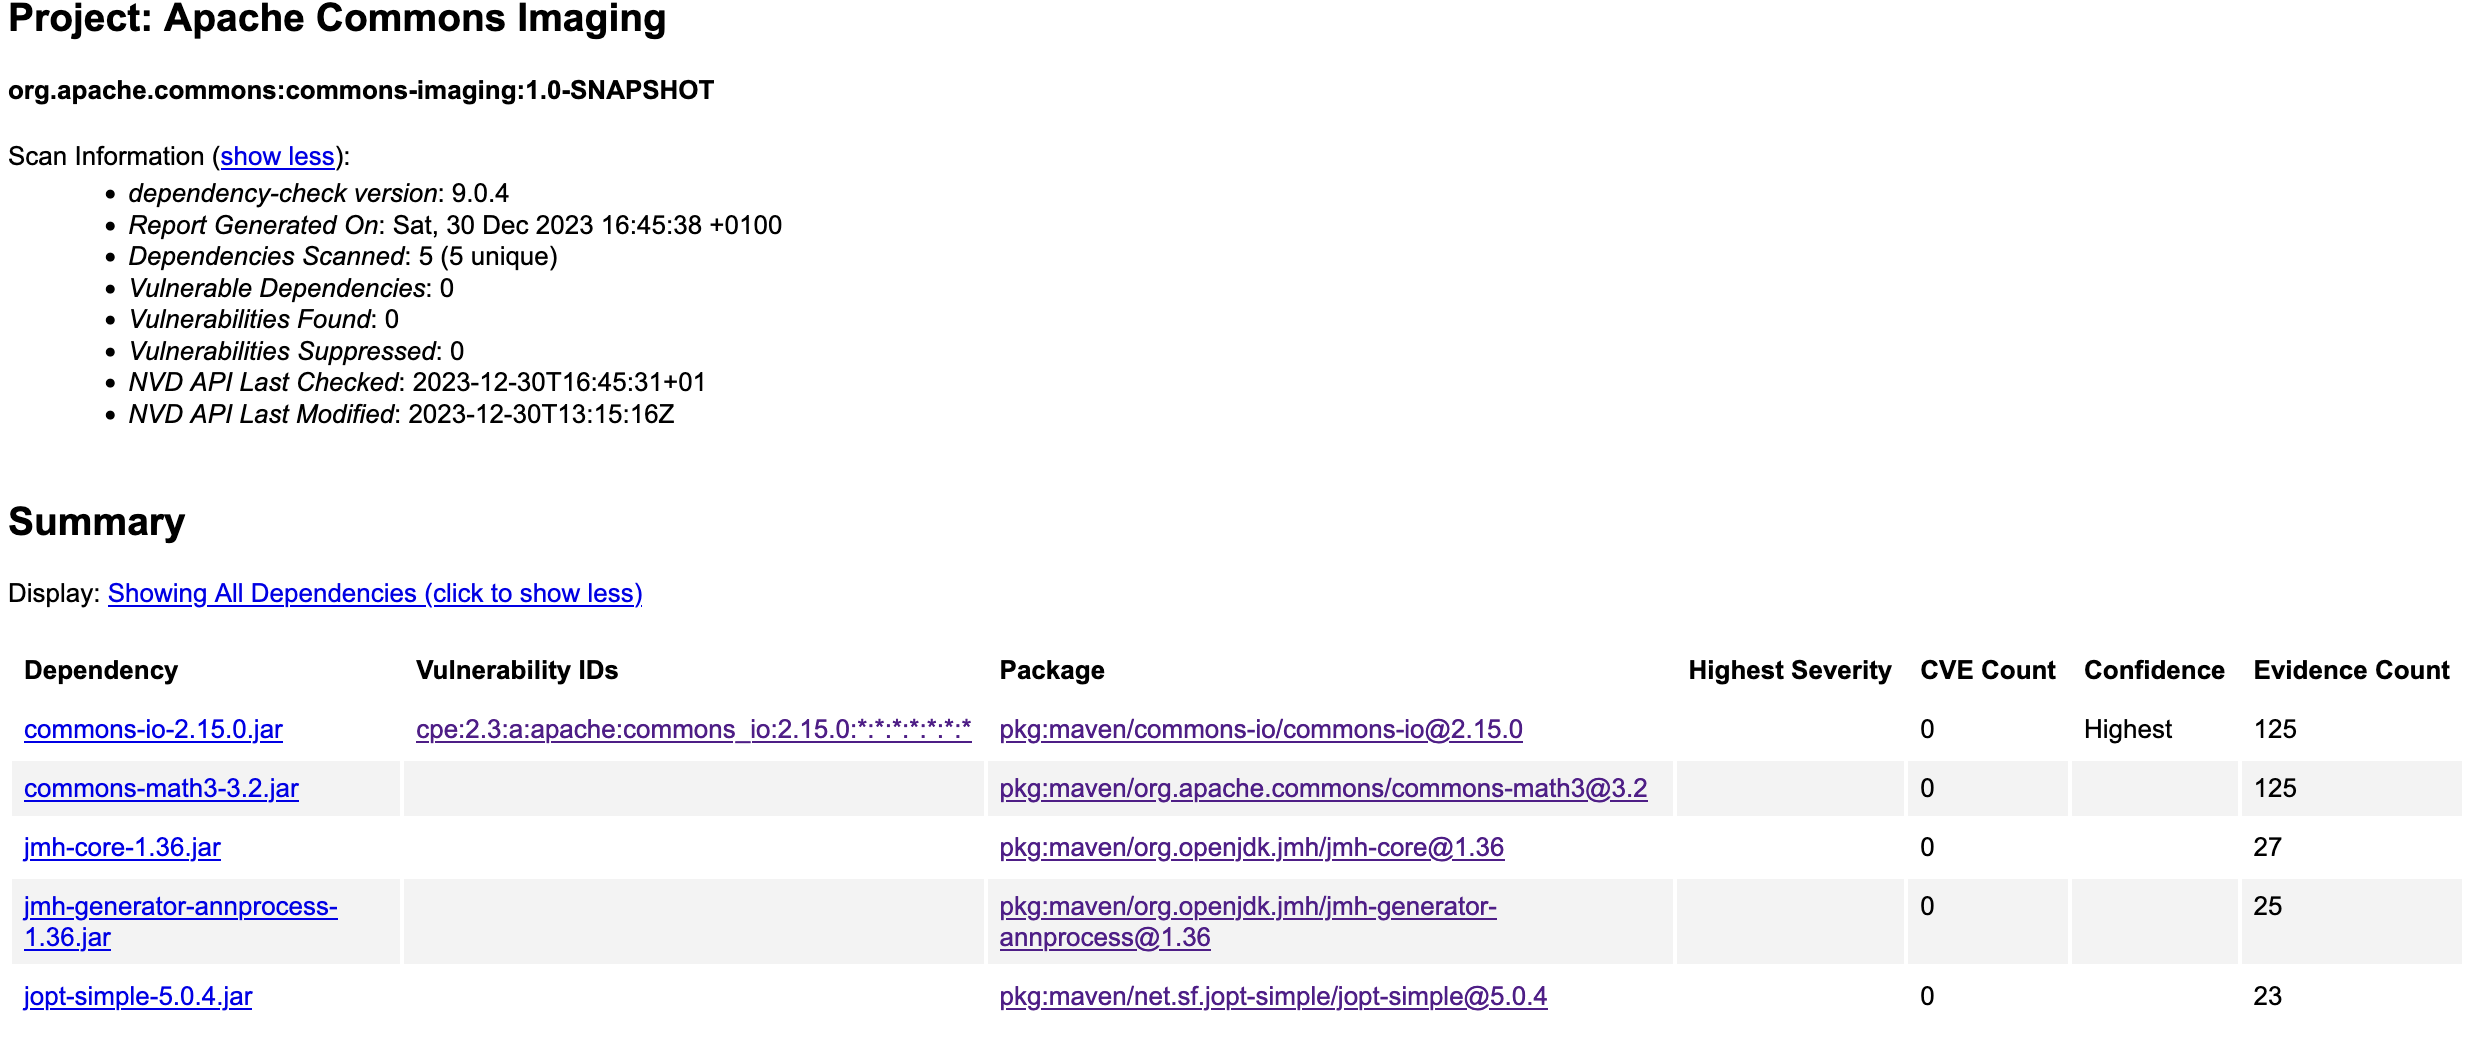
\includegraphics[width=1\linewidth,height=0.7\linewidth]{reportOwaspDC.png}
    \caption{Owasp DC - HTML Generated Report}
    \label{fig:enter-label}
\end{figure}


\subsection{Summary of Findings}

\begin{itemize}
    \item \textbf{Commons IO 2.15.0:}
        \begin{itemize}
            \item Description: The Apache Commons IO library contains utility classes, stream implementations, file filters, file comparators, endian transformation classes, and much more.
            \item \textbf{Analysis}: The analysis indicates a high-confidence dependency.
        \end{itemize}
    
    \item \textbf{Commons Math3 3.2:}
        \begin{itemize}
            \item Description: The Math project is a library of lightweight, self-contained mathematics and statistics components addressing the most common practical problems not immediately available in the Java programming language or commons-lang.
            \item \textbf{Analysis}: The analysis indicates a high-confidence dependency.
        \end{itemize}
    
    \item \textbf{JMH Core 1.36:}
        \begin{itemize}
            \item Description: This library constitutes the JMH Core for Java Microbenchmarking Harness. It is referenced in the project scope of Apache Commons Imaging, version 1.0-SNAPSHOT.
            \item \textbf{Analysis}: The analysis indicates a high-confidence dependency.
        \end{itemize}
    
    \item \textbf{JMH Generator Annprocess 1.36:}
        \begin{itemize}
            \item Description: This dependency represents the JMH Benchmark Generator based on Annotation Processors. Similar to the previous dependency, it is referenced in the project scope of Apache Commons Imaging, version 1.0-SNAPSHOT.
            \item \textbf{Analysis}: The analysis indicates a high-confidence dependency.
        \end{itemize}
    
    \item \textbf{Jopt Simple 5.0.4:}
        \begin{itemize}
            \item Description: Serving as a Java library for parsing command line options, this dependency is referenced in the project scope of Apache Commons Imaging, version 1.36.
            \item \textbf{Analysis}: The analysis indicates a high-confidence dependency.
        \end{itemize}
\end{itemize}

\subsection{Implications}

Owasp Dependency Checker doesn't report any vulnerabilities associated to the dependencies of the project. In the case of presence of vulnerabilities in these dependencies would underscore the critical importance of addressing and mitigating potential security risks. A proactive approach to dependency management and continuous monitoring is recommended to uphold the project's overall integrity and security posture.

These findings serve as a basis for further investigation and remediation efforts to enhance the robustness of the project's software supply chain.


\subsection{FindSecBugs (SpotBug)}

We conducted the analysis with FindSecBugs and identified two security bugs related to hard-coded keys. 

\begin{figure}[h!]
    \centering
    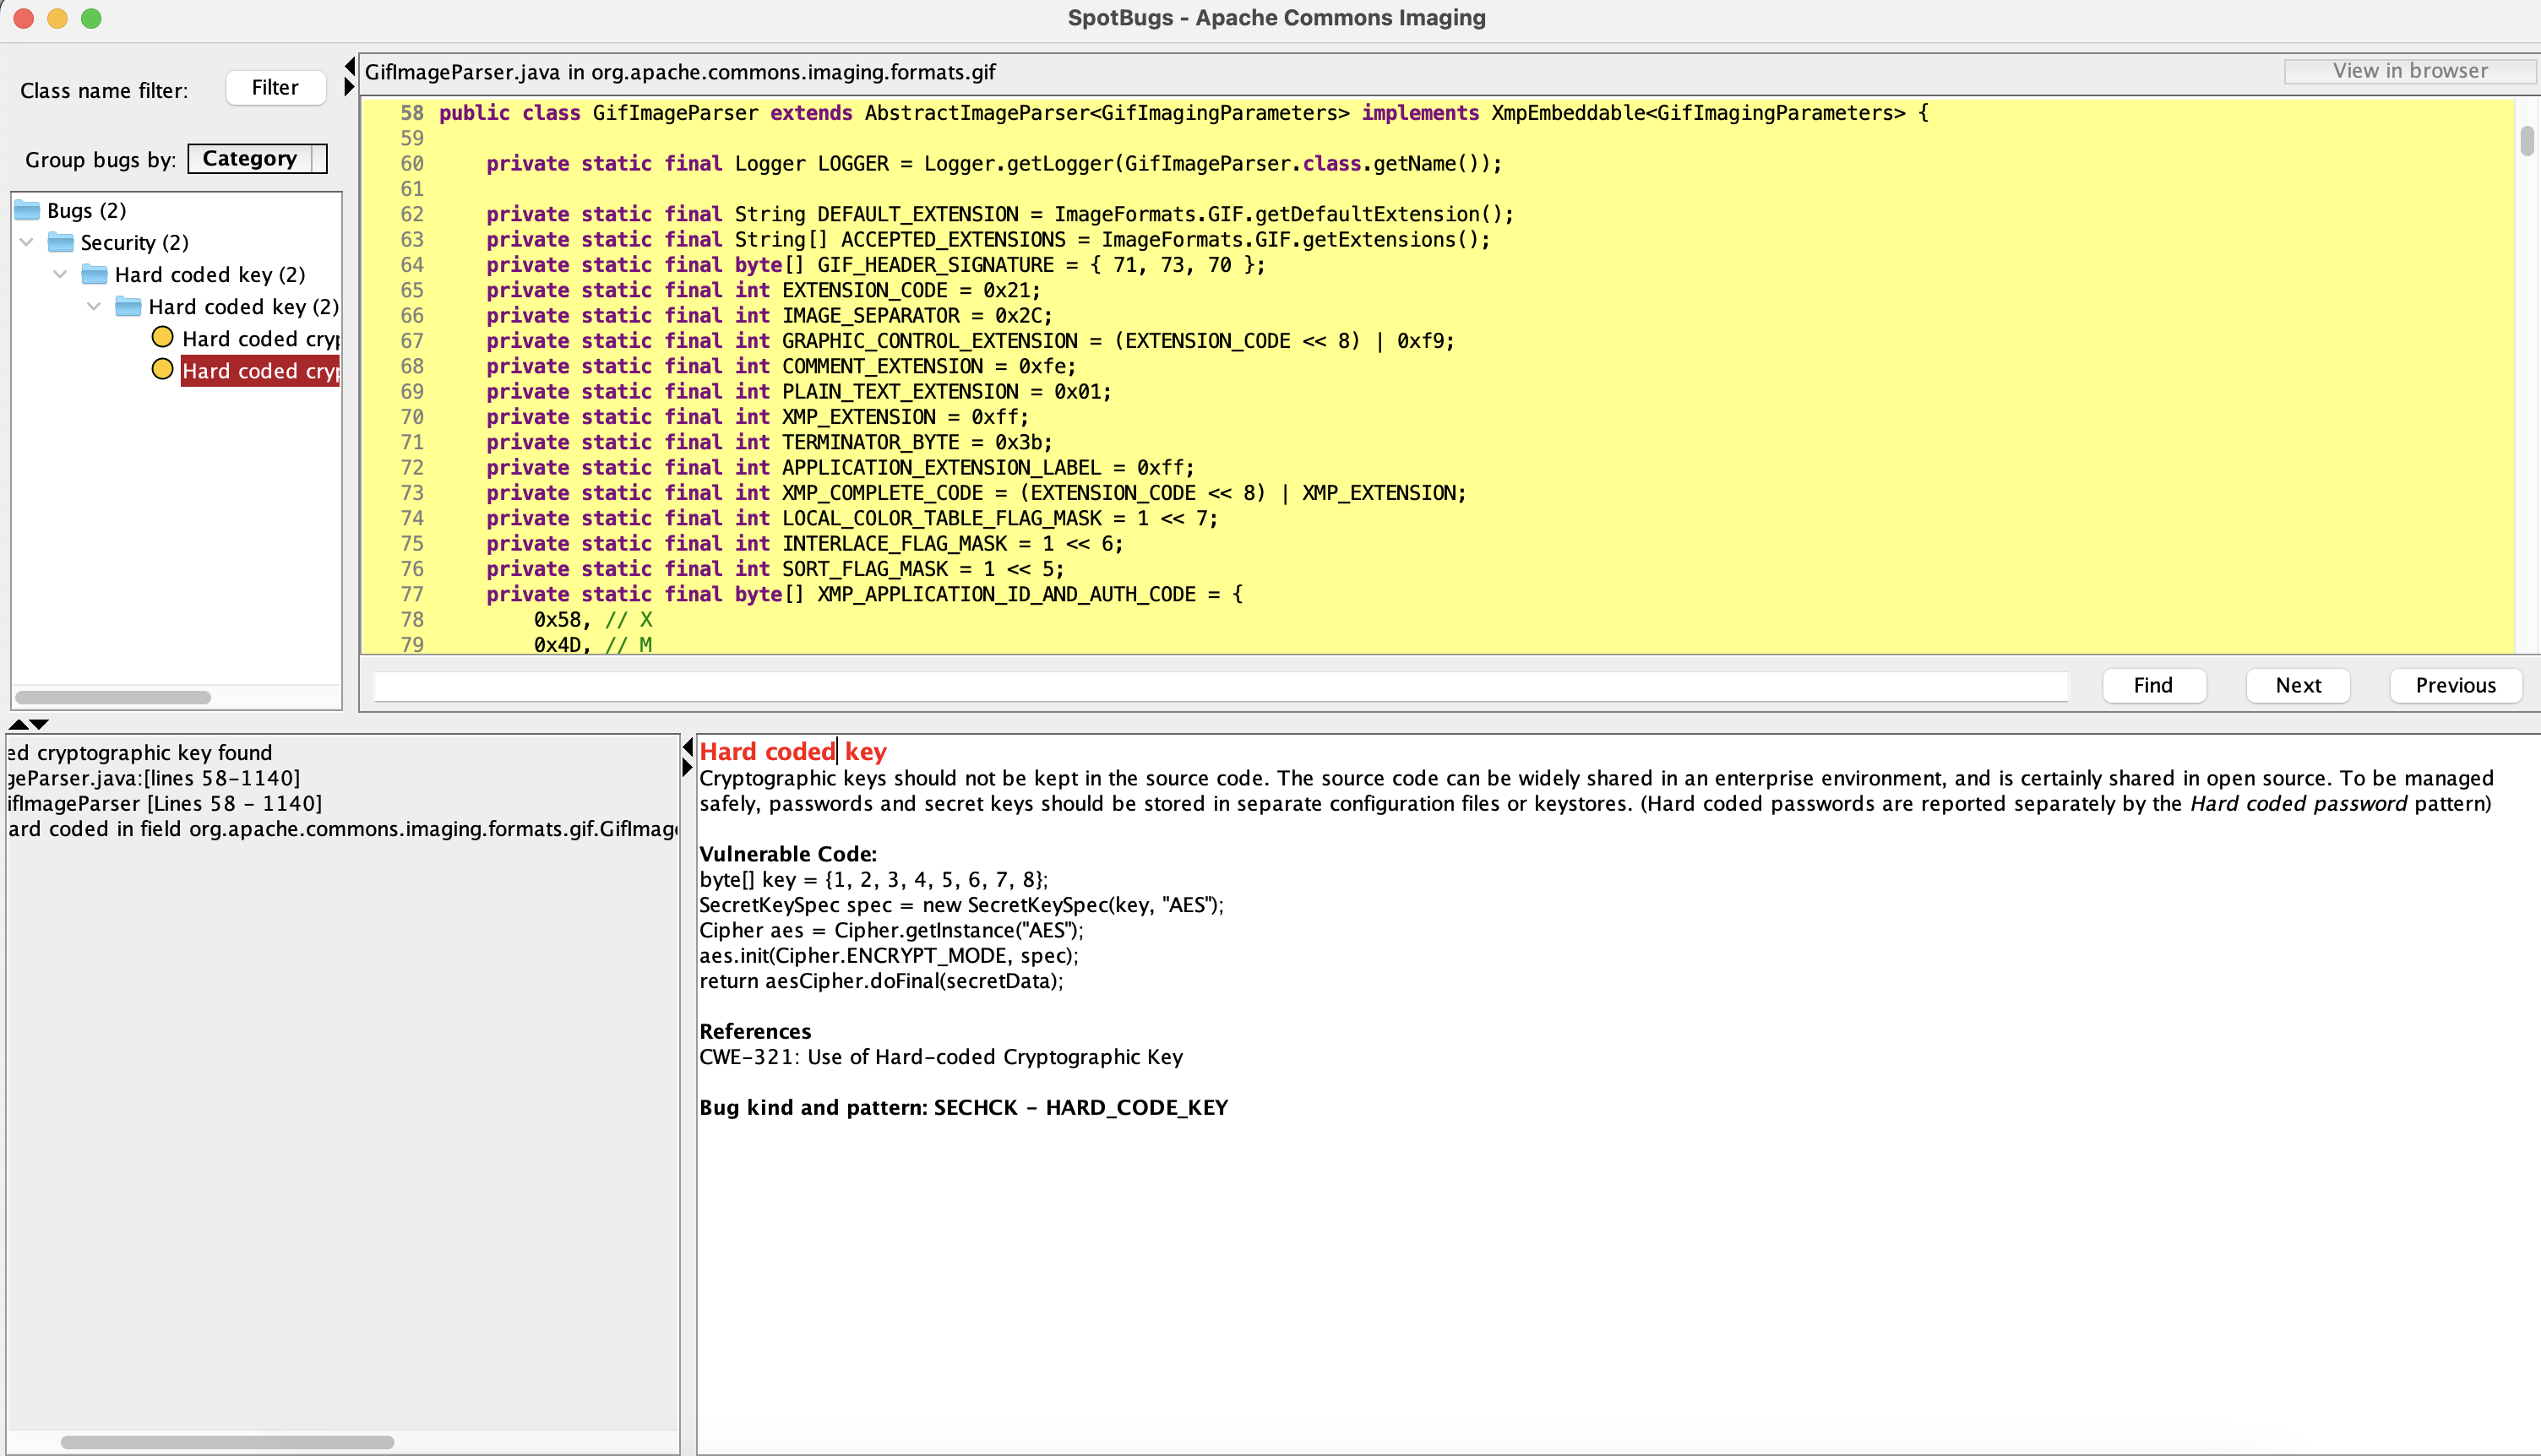
\includegraphics[width=1\linewidth]{reportFindSecBugs.png}
    \caption{Report before fix}
    \label{fig:enter-label}
\end{figure}

FindSecBugs references these types of vulnerabilities as the inappropriate storage of cryptographic keys in the source code. Given that source code can be widely distributed, especially in enterprise or open-source environments, it is not secure to include passwords and secret keys directly in the code. For secure management, passwords and secret keys should be stored in separate configuration files or keystores. (Note: Hard-coded passwords are addressed separately through the Hard-coded password pattern)

\section{Discussion}
TODO

\section{Conclusion}
TODO

%%
%% The acknowledgments section is defined using the "acks" environment
%% (and NOT an unnumbered section). This ensures the proper
%% identification of the section in the article metadata, and the
%% consistent spelling of the heading.
\begin{acks}
To the group, for always bringing "mate" while working.
\end{acks}

%% -> REFERENCES Section --> sample-base.bib has the cite references descriptions.
%% The next two lines define the bibliography style to be used, and
%% the bibliography file.

\bibliographystyle{ACM-Reference-Format}
\bibliography{sample-base}

%%
%% If your work has an appendix, this is the place to put it.
\appendix

\section{Research Methods}

\subsection{Part One}
TODO

\section{Online Resources}
TODO

\end{document}